\chapter{仿真}
\label{chapter:simu}

\section{概述}

\begin{figure}
\centering
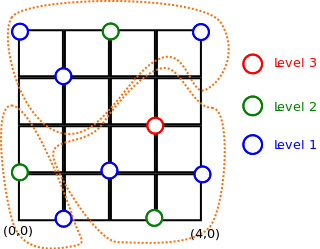
\includegraphics[width=4.5in]{png/paper-topo.png}
\caption{5x5网格型拓扑和产生的属性拓扑}
\label{fig:paper_topo}
\end{figure}

我们在ndnSIM上实现了TreeSync的仿真。
ndnSIM是Network Simulation(NS3)的一个模块,用于提供一个NDN的IP层的包装。
作为对比,我们同样实现了一个ChronoSync的ndnSIM版本。
在这一章中,我们首先验证逻辑的正确性和功能的实现。
然后我们在overhead和传输时延上做评估。

使结果更具一般性,我们采用如图\ref{fig:paper_topo}的5x5的网格拓扑结构。
网格中的每一个节点都代表一个参与者,所以总共更有25个节点。
拓扑图可能看起来很简单,但是实际上它包含6种不同环境中的节点,最大8跳的路由。
我们认为这个拓扑可以很好的代表一个一般的脱兔结构。
树形拓扑按照之前描述的算法生成。
所有的链路都具有10ms的延迟和1Mbps的带宽。
我们让参与者随机的生成新的数据,并且我们改变他们生成数据的频率来研究变化趋势。
每个人产生信息的周期是独立的。

\section{功能实现}

\begin{figure}
\centering
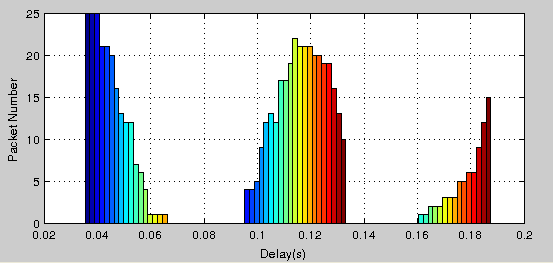
\includegraphics[width=4.5in]{png/function-delay.png}
\caption{节点收到数据的延迟}
\label{fig:function_delay}
\end{figure}

1.控制节点产生。
在网格拓扑中,控制节点产生像预期一样工作。
产生了一个四层的拓扑,最高级的控制节点在节点(3,2)上。

2.消息同步。
所有的消息都能够成功的传递给聊天室的所有人,不会丢失任何消息。
图\ref{fig:function_delay}显示了当产生频率为$2/7Hz$时的时延。从图中可以看出,时延被分为三个部分。
很快,平均,和稍慢。这是和树形拓扑紧密相关的。
如果接收者在消息产生者很近的位置,他们在树形拓扑中也会距离很近,这样他就能够很快得到控制信息,进而获取实际消息实体。
然而,当两个参与者在树形拓扑中相距很远时,控制信息要跨越好几个层级才能到达,导致了相对更大的时延。


\section{效果评估}

\subsection{链路负载}

\begin{figure}
\centering
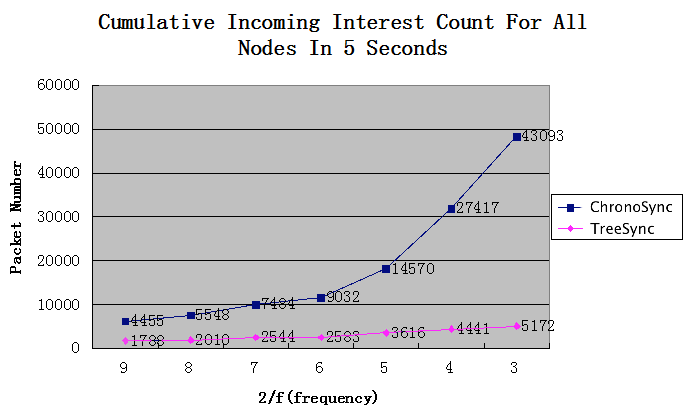
\includegraphics[width=4.5in]{png/all-incoming-interest-revised.png}
\caption{所有节点的进入的兴趣包数目}
\label{fig:overhead}
\end{figure}
\begin{figure}
\centering
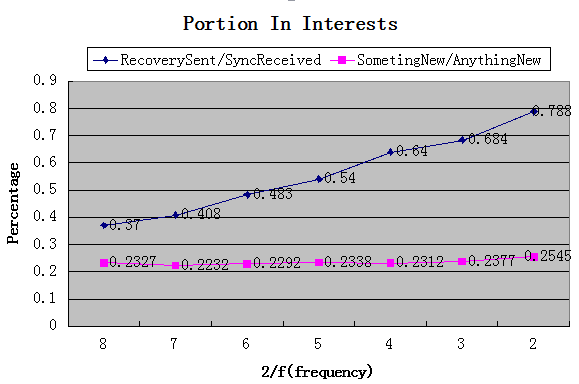
\includegraphics[width=4.5in]{png/portion-in-interests.png}
\caption{兴趣包中不同成分所占的比例}
\label{fig:interest_percentage}
\end{figure}

我们的设计在控制性上面有很大的优势,所以在overhead上会比ChronoSync有显著的减少。
在我们的试验中,我们改变消息声称的平率,然后观察overhead的变化。
在图\ref{fig:overhead}中,当频率增加时,我们的设计在包数统计上会有线性的增加,然而ChronoSync却遭受了指数的增长。
这是因为当产生消息的频率增加时,同时产生消息的频率也指数增加,那么ChronoSync就必须发送额外的恢复兴趣包来处理这种冲突。
注意到我们使用的是所有进入的兴趣包的数目统计,因为它可以代表整个状态。
NDN路由器的聚合性也可以减少进入的兴趣包数。
从图\ref{fig:interest_percentage}可以看出,
在ChronoSync中节点需要发送恢复兴趣包的比例随着频率增长得非常快,
然而在我们的设计中,SNI和ANI的比例基本保持不变。

\subsection{延迟}

\begin{figure}
\centering
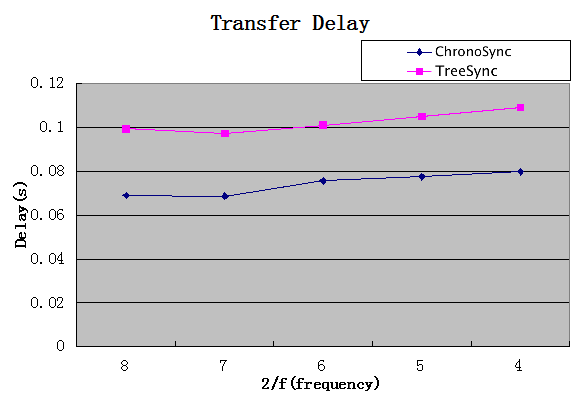
\includegraphics[width=4.5in]{png/delay-compare-revised.png}
\caption{延迟比较}
\label{fig:delay_compare}
\end{figure}

\begin{figure}
\centering
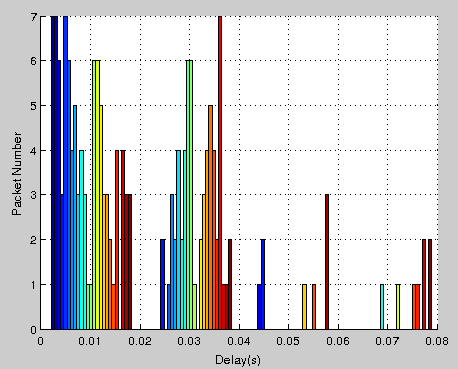
\includegraphics[width=4.5in]{png/data-fetch-delay.png}
\caption{数据获取兴趣包拉回数据的延迟}
\label{fig:data_fetch_delay}
\end{figure}

由于控制信息要经过多层控制器,即时拓扑结构和实际拓扑是紧密相关的,延迟效果依然比完全按照最有路径的ChronoSync稍差。
但是,当数据产生更加频繁时,ChronoSync需要发送更多的恢复兴趣包,并且当带宽不足时会增加其时延。
如图\ref{fig:delay_compare}所示,TreeSync的时延要稍大于ChronoSync,但是仍然很好,并且两种方法都大幅度优于IP网络模型解决方案。
考虑到获得的巨大的控制性能,这种权衡牺牲是值得的。

另一点,在我们的数据中,实际数据的获取是完全分布式的,可以充分利用NDN结构的优点。
图\ref{fig:data_fetch_delay}显示了参与者从发送实际消息请求到得到数据的延迟,可以看到这个过程非常迅速。
并且这种设计也为低时延和小overhead做出了贡献。
